\documentclass[aspectratio=169]{beamer}

\usetheme{Madrid}
\usecolortheme{default}
\setbeamertemplate{navigation symbols}{}
\setbeamertemplate{footline}{
  \leavevmode%
  \hbox{\begin{beamercolorbox}[wd=.333\paperwidth,ht=2.5ex,dp=1ex,center]{author in head/foot}%
    \usebeamerfont{author in head/foot}\insertshortauthor
  \end{beamercolorbox}%
  \begin{beamercolorbox}[wd=.333\paperwidth,ht=2.5ex,dp=1ex,center]{title in head/foot}%
    \usebeamerfont{title in head/foot}\insertshorttitle
  \end{beamercolorbox}%
  \begin{beamercolorbox}[wd=.333\paperwidth,ht=2.5ex,dp=1ex,right]{date in head/foot}%
    \insertframenumber/\inserttotalframenumber\hspace*{2ex}
  \end{beamercolorbox}}%
}

\usepackage{graphicx}
\usepackage{amsmath}
\usepackage{booktabs}
% tikz, algorithmic, xcolor, hyperref removed (loaded by beamer)

\graphicspath{{images/}}

\title[Lightweight Encryption]{Comparison of Lightweight Encryption Algorithms}
\subtitle{B.Tech Final Year Project}

\author[R. Jena, S. Kumar, P. Kumar]{
Rajesh Kumar Jena (B122088) \and
Soumil Kumar (B122114) \and
Punit Kumar (B422041)
}

\institute{
International Institute of Information Technology\\
Bhubaneswar\\
Supervisor: Prof. Debasish Jena
}

\date{May 2026}

\begin{document}

\begin{frame}
\titlepage
\end{frame}

\begin{frame}{Outline}
\tableofcontents
\end{frame}

\section{Introduction}

\begin{frame}{Motivation and Problem Statement}
\textbf{Historical Context}
\begin{itemize}
    \item DES (1977) $\rightarrow$ AES (2001): Evolved for desktop/server computing
    \item IoT devices: constrained CPU, memory, power — traditional algorithms impractical
    \item Mirai botnet (2016): Exploited insecure embedded devices --- millions hijacked
\end{itemize}

\vspace{0.2cm}
\textbf{Problem}
\begin{itemize}
    \item Developers deploy weakened or ad hoc security
    \item Lightweight cryptography: efficient primitives for constrained platforms
    \item Need to balance security, performance, and implementation cost
\end{itemize}
\end{frame}

\begin{frame}{Objectives \& Contributions}
This study aims to:
\begin{itemize}
    \item Evaluate PRESENT, SPECK, and ASCON on Raspberry Pi Pico (ARM Cortex-M0+)
    \item Compare execution time, memory usage, and throughput
    \item Identify design trade-offs for constrained embedded environments
\end{itemize}

\vspace{0.2cm}
\textbf{Contributions:}
\begin{itemize}
    \item Reproducible Rust-based benchmarking framework for RP2040
    \item Empirical data across block cipher, mode, and payload-size dimensions
    \item Practical deployment recommendations based on measured trade-offs
\end{itemize}
\end{frame}


\section{Experimental Methodology}

\begin{frame}{Algorithms: Design Properties}
\vspace{-0.4cm}
\begin{table}
    \centering
    \begin{tabular}{lccc}
        \toprule
        \textbf{Property} & \textbf{PRESENT} & \textbf{SPECK} & \textbf{ASCON} \\
        \midrule
        Block Size & 64 bits & 64 bits & 64 bits \\
        Key Sizes & 80, 128 bits & 64--256 bits & 128 bits \\
        Structure & SPN & ARX Feistel & Sponge-Duplex \\
        Rounds & 31/32 & 22-34 & 12 \\
        Standardization & ISO 29192-2 & --- & NIST SP 800-232 \\
        AEAD Support & No & No & Yes \\
        \bottomrule
    \end{tabular}
\end{table}

\vspace{0.15cm}
\textbf{Key Differentiators}:
\begin{itemize}
    \item \textbf{PRESENT}: $\sim$1,570 GE (hardware-optimized)
    \item \textbf{SPECK}: 42 CPB (software fastest)
    \item \textbf{ASCON}: AEAD + hashing built-in
\end{itemize}
\end{frame}

\begin{frame}{Platform \& Metrics}
\textbf{Hardware}: Raspberry Pi Pico (ARM Cortex-M0+, 133 MHz, 264 KB SRAM)

\vspace{0.15cm}
\textbf{Metrics}: Throughput (Mbps), Cycles/Byte, ROM footprint, RAM usage

\vspace{0.15cm}
\textbf{Procedure}: 1000+ iterations, hardware timer, test vector validation
\end{frame}


\section{Results}

\begin{frame}{Block Cipher Benchmarks}
\vspace{-0.3cm}
\begin{table}
    \centering
    \begin{tabular}{lrr}
        \toprule
        \textbf{Algorithm} & \textbf{CPB} & \textbf{Mbps} \\
        \midrule
        PRESENT-80 & $2{,}958$ & 0.34 \\
        PRESENT-128 & $3{,}068$ & 0.33 \\
        SPECK-64/96 & 42 & 23.81 \\
        SPECK-64/128 & 42 & 23.67 \\
        ASCON-128 & 132 & 7.56 \\
        \bottomrule
    \end{tabular}
\end{table}
\vspace{0.1cm}
\textbf{Key Finding}: SPECK is \textbf{70x faster} than PRESENT and \textbf{3x faster} than ASCON.
\end{frame}

\begin{frame}{Why This Performance Gap?}
\textbf{Architectural Explanation:}
\begin{itemize}
    \item \textbf{SPECK (ARX)}: Add, Rotate, XOR $\rightarrow$ single-cycle ARM instructions (\texttt{ADDS}, \texttt{RORS}, \texttt{EORS}) — no memory lookups
    \item \textbf{PRESENT (SPN)}: Bit-permutation requires 64 separate bit extractions/reinsertions per round — 31 rounds (PRESENT-80) / 32 rounds (PRESENT-128) = 70x overhead
    \item \textbf{ASCON (Sponge)}: 64-bit words align with Cortex-M0+ datapath, but 12-round $p^a$ permutation is heavier than SPECK's 5-instruction round
\end{itemize}

\vspace{0.2cm}
\textbf{Bottom Line}: Hardware-optimized ciphers (PRESENT) sacrifice software performance; software-optimized ciphers (SPECK) exploit architectural fit.
\end{frame}

\begin{frame}{Memory Footprint}
\vspace{-0.3cm}
\begin{table}
    \centering
    \begin{tabular}{lrrrr}
        \toprule
        \textbf{Cipher} & \textbf{Key} & \textbf{State} & \textbf{ROM} & \textbf{RAM} \\
        \midrule
        PRESENT-80 & 80 bits & 8 bytes & $\sim$2 KB & $\sim$16 B \\
        PRESENT-128 & 128 bits & 8 bytes & $\sim$2.5 KB & $\sim$16 B \\
        SPECK-64/96 & 96 bits & 16 bytes & $\sim$1 KB & $\sim$32 B \\
        SPECK-64/128 & 128 bits & 16 bytes & $\sim$1.2 KB & $\sim$32 B \\
        ASCON-128 & 128 bits & 40 bytes & $\sim$3 KB & $\sim$40 B \\
        \bottomrule
    \end{tabular}
\end{table}
\vspace{0.2cm}
\textbf{SPECK}: Smallest ROM ($\sim$1 KB) — ARX-only ops, no lookup tables
\end{frame}

\begin{frame}{ASCON Phase Breakdown}
\vspace{-0.3cm}
\begin{columns}
\begin{column}{0.45\textwidth}
\begin{table}
    \centering
    \begin{tabular}{lr}
        \toprule
        \textbf{Phase} & \textbf{Cycles} \\
        \midrule
        Initialization & 427 \\
        Absorb (AD) & 216 \\
        Encrypt & 464 \\
        Finalize & 422 \\
        \midrule
        \textbf{Total} & \textbf{1{,}529} \\
        \bottomrule
    \end{tabular}
\end{table}
\end{column}
\begin{column}{0.50\textwidth}
\centering
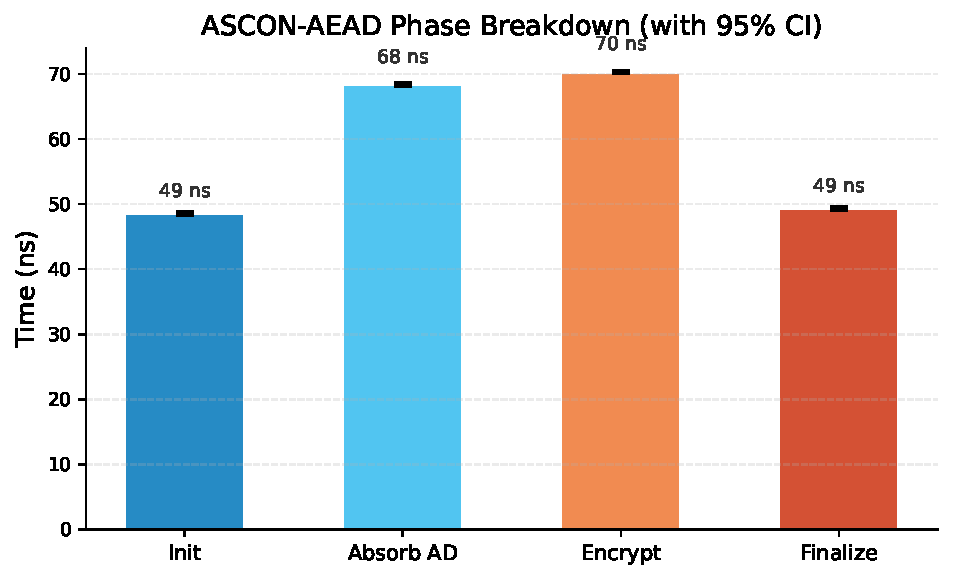
\includegraphics[width=1.0\textwidth]{ascon_phases.pdf}
\end{column}
\end{columns}
\end{frame}

\begin{frame}{Energy Efficiency (µJ/byte)}
\begin{table}
    \centering
    \begin{tabular}{lrrrr}
        \toprule
        \textbf{Cipher} & \textbf{16B} & \textbf{64B} & \textbf{256B} & \textbf{1024B} \\
        \midrule
        SPECK-64/128 (CTR) & 0.29 & 0.27 & 0.26 & 0.25 \\
        ASCON-128 (AEAD) & 2.56 & 0.64 & 0.51 & 0.47 \\
        PRESENT-128 (CTR) & 27.18 & 27.07 & 27.17 & 27.00 \\
        \bottomrule
    \end{tabular}
\end{table}
\vspace{-0.2cm}
\begin{itemize}
    \item SPECK: 108x more energy-efficient than PRESENT
    \item ASCON: $\sim$41 µJ initialization overhead (constant), but per-byte cost scales from 2.56→0.47 µJ as payload grows
    \item Ideal for battery-powered IoT sensors
\end{itemize}
\end{frame}

\begin{frame}{Speedup Analysis}
\begin{columns}[T]
\begin{column}{0.40\textwidth}
Performance relative to ASCON:
\vspace{0.1cm}
\begin{table}
    \centering
    \small
    \begin{tabular}{lccc}
        \toprule
        \textbf{Cipher} & \textbf{64B} & \textbf{256B} & \textbf{1024B} \\
        \midrule
        SPECK (ECB) & 1.34x & 1.08x & 1.03x \\
        PRESENT & 0.012x & 0.010x & 0.009x \\
        \bottomrule
    \end{tabular}
\end{table}
\vspace{0.15cm}
\textbf{Insight}: ASCON's 427-cycle init overhead amortizes at larger payloads; SPECK advantage shrinks from 34\% to 3\%.
\end{column}
\begin{column}{0.55\textwidth}
\centering
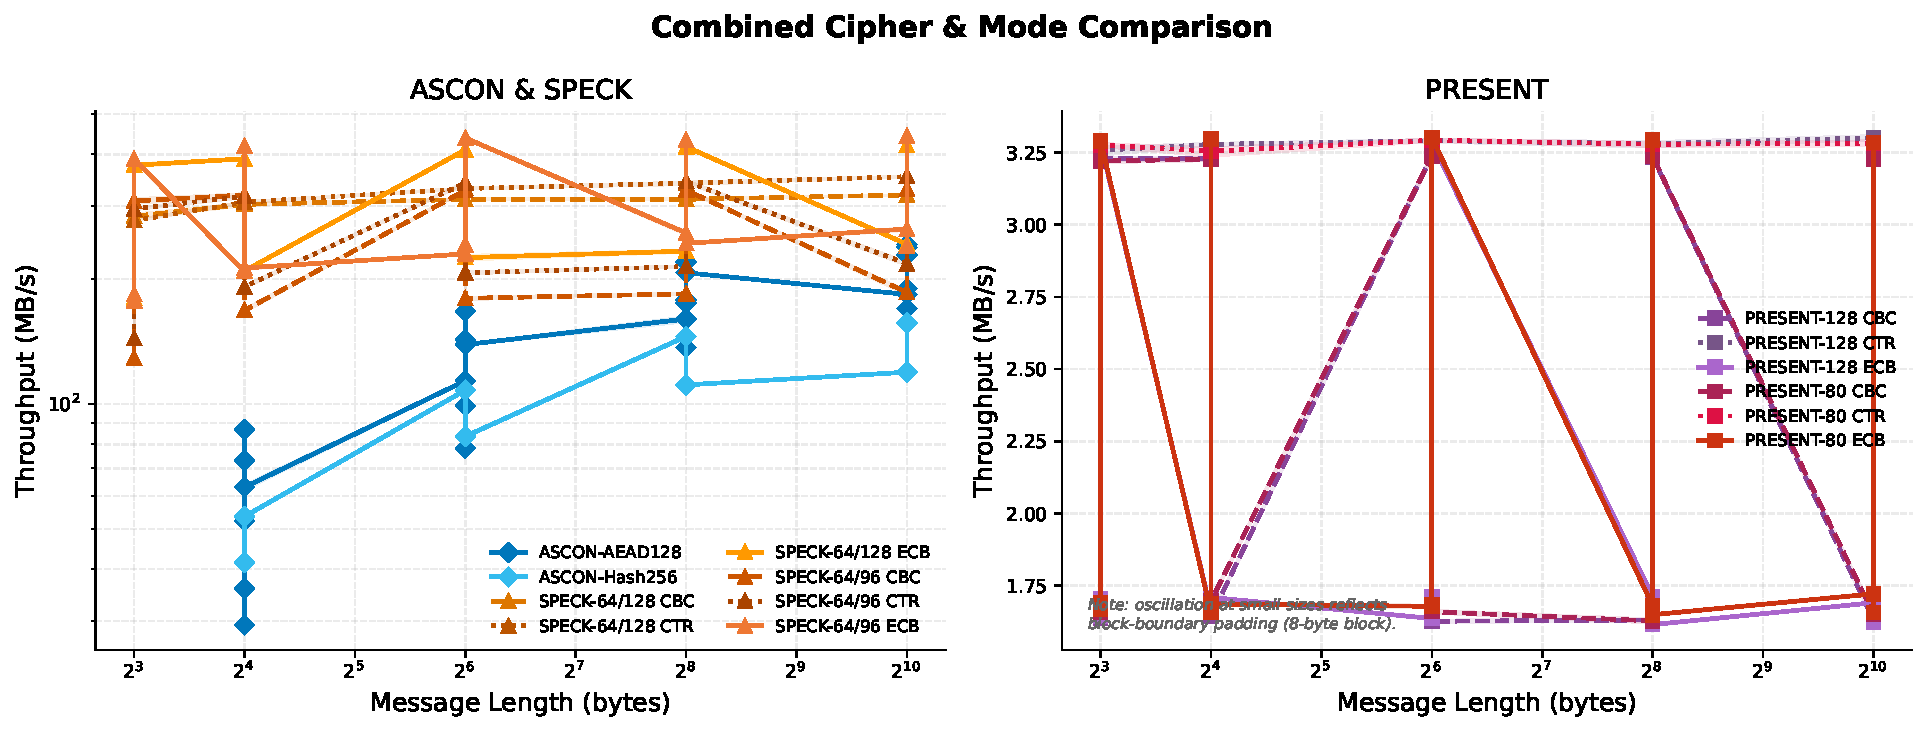
\includegraphics[width=0.9\textwidth]{combined_comparison.pdf}
\end{column}
\end{columns}
\end{frame}


\section{Analysis}

\begin{frame}{Scorecard Comparison}
\vspace{-0.3cm}
\begin{table}
    \centering
    \begin{tabular}{lccc}
        \toprule
        \textbf{Metric} & \textbf{PRESENT} & \textbf{SPECK} & \textbf{ASCON} \\
        \midrule
        Throughput (Mbps) & 0.34 & 23.67 & 7.56 \\
        CPB (cycles) & $2{,}958$ & 42 & 132 \\
        ROM (KB) & 2.5 & 1.2 & 3.0 \\
        RAM (bytes) & 16 & 32 & 40 \\
        AEAD & No & No & Yes \\
        NIST Standard & No & No & Yes \\
        ISO Standard & Yes & No & No \\
        \bottomrule
    \end{tabular}
\end{table}
\end{frame}

\begin{frame}{Security Considerations}
\begin{itemize}
    \item \textbf{ASCON}: NIST SP 800-232, proven indifferentiability bounds, no attacks on full 12-round permutation
    \item \textbf{PRESENT}: ISO/IEC 29192-2, provable SPN bounds (max diff probability $2^{-2}$), confidentiality only
    \item \textbf{SPECK}: No provable bounds, best attacks reduce 20/27 rounds; ISO rejection (NSA origin, geopolitical objections)
    \item \textbf{Side-channels}: SPECK vulnerable to CPA (50 traces on 8-bit); PRESENT's constant-time ops more resistant
\end{itemize}
\end{frame}


\section{Recommendations}

\begin{frame}{Use-Case Recommendations}
\begin{enumerate}
    \item \textbf{Real-time sensor data}: SPECK-64/128 (CTR) — 23.67 Mbps, 32B RAM
    \item \textbf{Secure IoT with auth}: ASCON — 7.56 Mbps, AEAD, NIST standardized
    \item \textbf{RFID tags}: PRESENT — ultra-low gate count (~1570 GE)
    \item \textbf{Firmware authentication}: ASCON-hash — 320-bit state, 12-round $p^a$
    \item \textbf{Hybrid deployment}: SPECK (bulk) + ASCON (auth tags)
    \item \textbf{Legacy integration}: PRESENT-128 (CBC) — backward compatibility
\end{enumerate}
\end{frame}

\begin{frame}{Limitations \& Future Work}
\begin{itemize}
    \item \textbf{Side-channels}: Not analyzed; SPECK shows vulnerability to CPA attacks
    \item \textbf{Scope}: Single platform (RP2040), software-only implementations
    \item \textbf{Future}: Hardware-accelerated implementations, side-channel countermeasures
\end{itemize}
\end{frame}

\begin{frame}[plain]
\begin{center}
\Huge Thank You\\[0.8cm]
\normalsize Rajesh Kumar Jena (B122088)\\
Soumil Kumar (B122114)\\
Punit Kumar (B422041)\\[0.5cm]
\end{center}
\end{frame}

\end{document}